\documentclass[review,12pt]{elsarticle}

\usepackage{amsmath,amssymb,amsfonts}
\usepackage{graphicx}
\usepackage{booktabs}
\usepackage{hyperref}
\usepackage{cleveref}
\usepackage{microtype}
\usepackage{siunitx}
\usepackage{subcaption}
\usepackage{multirow}
\usepackage{xcolor}
\usepackage{algorithm}
\usepackage{algpseudocode}
\usepackage[margin=2.5cm]{geometry}

\journal{Sensors and Actuators A: Physical}

%% ─────────────────────────────────────────────────────────────────────────────
\begin{document}

\begin{frontmatter}

\title{A Deep Ritz Physics-Informed Neural Network for Large-Deflection Modelling
       of Multilayer Parylene-C/Au/Parylene-C MEMS Diaphragm Pressure Sensors}

\author[metu]{Seckin Eroglu}
\author[metu]{Ender Yildirim\corref{cor1}}
\cortext[cor1]{Corresponding author. Tel.: +90-312-210-XXXX.}
\ead{eyildirim@metu.edu.tr}

\address[metu]{Department of Electrical and Electronics Engineering,
               Middle East Technical University, 06800 Ankara, Turkey}

%% ─────────────────────────────────────────────────────────────────────────────
\begin{abstract}
Accurate and fast modelling of large-deflection behaviour in MEMS capacitive
pressure sensors is a prerequisite for design optimisation and real-time
performance prediction. Classical Kirchhoff plate theory (Atik analytical
model) systematically overestimates deflection at operating pressures because
it neglects membrane stiffening; full finite-element analysis (FEA) is accurate
but prohibitively slow for high-throughput design exploration. We present
\emph{MEMSRitz}, an energy-driven physics-informed neural network (PINN) based
on the Deep Ritz method that learns the equilibrium deflection and radial
in-plane displacement of a clamped circular multilayer
parylene-C\,/\,gold\,/\,parylene-C diaphragm over a five-dimensional geometry
space ($a \in [150,500]$\,\si{\micro\metre},
$a_\mathrm{g} \in [5,15]$\,\si{\micro\metre}, layer thicknesses
$t_1,t_3\in[1,5]$\,\si{\micro\metre},
$t_2\in[0.2,0.5]$\,\si{\micro\metre}) and a three-decade pressure range
($P\in[10,20\,000]$\,Pa). The network is trained by minimising the
Föppl–von Kármán (FvK) variational energy functional—no labelled FEA data
are required in the main training phase. Classical Laminated Plate Theory (CLT)
provides the bending stiffness $D^*$ and membrane stiffness $A_{11}$,
$A_{12}$ analytically for each geometry. Hard clamped boundary conditions are
enforced algebraically via the shape factor $(1-\xi^2)^2$, and electrode
contact ($w \ge -a_\mathrm{g}$) is guaranteed by a smooth-max operator in the
forward pass. Validated against 2144 COMSOL FEA profiles, the model achieves a
median RMSE of \SI{0.15}{\micro\metre} and a maximum of \SI{1.10}{\micro\metre},
with zero contact-penetration violations, while reducing inference time from
minutes (FEA) to sub-millisecond. The Kirchhoff analytical model is shown to
overestimate centre deflection by 20–50\% above \SI{2}{\kilo\pascal},
confirming the necessity of the full FvK treatment captured by the network.
\end{abstract}

\begin{keyword}
MEMS pressure sensor \sep
parylene-C diaphragm \sep
physics-informed neural network \sep
Deep Ritz method \sep
Föppl–von Kármán \sep
Classical Laminated Plate Theory \sep
touch mode capacitive sensor \sep
surrogate model
\end{keyword}

\end{frontmatter}

%% ─────────────────────────────────────────────────────────────────────────────
\section{Introduction}
\label{sec:intro}

Capacitive MEMS pressure sensors based on thin circular diaphragms have become
the workhorse transducer architecture for biomedical implants, environmental
monitoring, and industrial process control
\cite{fragiacomo2010,lo2007,sim2005}. The device of interest in this work is
built around a three-layer stack of parylene-C / gold / parylene-C: the two
polymer layers form the flexible structural membrane while the gold interlayer
provides the conducting electrode and contributes disproportionately to the
bending stiffness through an I-beam effect. At physiologically and
industrially relevant pressures (tens of Pa to tens of kPa), the ratio of
centre deflection to layer thickness routinely exceeds unity, placing the
device firmly in the geometrically nonlinear large-deflection regime. In this
regime the classical Kirchhoff (linear) plate solution—which underlies the
widely used analytical model of Atik et al.~\cite{atik2020}—systematically
overestimates deflection because it ignores in-plane membrane stiffening, a
central prediction of Föppl–von Kármán (FvK) theory.

Accurate large-deflection analysis via FEA (e.g.\ COMSOL Multiphysics) resolves
this nonlinearity but at the cost of minutes to hours per geometry–pressure
evaluation. Design space exploration and sensor calibration routinely require
$10^3$–$10^4$ such evaluations, making full FEA intractable as an inner loop.
Surrogate models trained on FEA data can reduce this cost but require large
labelled datasets that are expensive to generate and that do not generalise
automatically beyond the training distribution
\cite{zacchei2024,dibarba2022}.

Physics-informed neural networks (PINNs) offer an alternative: instead of
fitting labelled outputs, the network is trained by minimising a physics
residual derived from the governing equations
\cite{raissi2019,lagaris1998,karniadakis2021}.  In their variational form,
PINNs minimise the total potential energy, recovering the governing PDEs as
Euler–Lagrange conditions of the energy functional. This approach—the
\emph{Deep Ritz method}~\cite{e2018}—was introduced for general variational
problems and subsequently extended to nonlinear mechanics
\cite{samaniego2020,fuhg2022}.  Recent applications to plate and shell
structures~\cite{wangThai2025} have demonstrated that Deep Ritz formulations
can match FEA accuracy while operating without labelled training data.

Despite this progress, no study has applied a Deep Ritz PINN to the specific
geometry and physics of a multilayer MEMS capacitive diaphragm: a
clamped circular FvK plate with electrode contact, composite (CLT) stiffness,
and a geometry space spanning multiple orders of magnitude in both dimensions
and pressure. The challenges are threefold. First, the five-dimensional
geometry space must be represented compactly. Second, electrode contact
($w \ge -a_\mathrm{g}$) is a \emph{hard} unilateral constraint; soft penalty
approaches are known to fail at large pressure ratios
\cite{e2018,samaniego2020}. Third, the energy scales of individual samples span
four orders of magnitude across the pressure range, making naive energy
minimisation biased toward high-pressure samples.

This paper addresses all three challenges. The contributions are:
\begin{enumerate}
    \item A Deep Ritz PINN architecture with two output heads—transverse
          deflection $w(r)$ and in-plane displacement $u(r)$—parameterised over
          the full five-dimensional geometry and three-decade pressure space.
    \item Algebraic enforcement of clamped boundary conditions via the
          shape factor $(1-\xi^2)^2$, eliminating any gradient budget spent on
          boundary residuals.
    \item A smooth-max operator in the network forward pass that enforces
          electrode contact to within \SI{50}{nm} with nonzero gradient
          everywhere, enabling the network to learn touch-mode physics.
    \item A per-sample energy normalisation scheme that equalises gradient
          contributions across the full pressure range.
    \item Validation against 2144 COMSOL deflection profiles, demonstrating
          median RMSE of \SI{0.15}{\micro\metre} and sub-millisecond inference.
\end{enumerate}

The paper is organised as follows. Section~\ref{sec:physics} describes the
device geometry and the FvK energy functional. Section~\ref{sec:network}
presents the neural network architecture and training strategy. Results are
given in Section~\ref{sec:results} and discussed in
Section~\ref{sec:discussion}. Conclusions follow in
Section~\ref{sec:conclusion}.

%% ─────────────────────────────────────────────────────────────────────────────
\section{Physical Model}
\label{sec:physics}

\subsection{Device geometry}
\label{sec:device}

The sensor consists of a clamped circular diaphragm of radius $a$ suspended
above a fixed bottom electrode, separated by an initial air gap $a_\mathrm{g}$
(\cref{fig:schematic}). The diaphragm is a three-layer laminate:
\begin{itemize}
    \item Layer 1: parylene-C, thickness $t_1$, Young's modulus
          $E_p = \SI{3.2}{\giga\pascal}$, Poisson's ratio $\nu_p = 0.33$
    \item Layer 2: gold, thickness $t_2$, $E_\mathrm{Au} = \SI{70}{\giga\pascal}$,
          $\nu_\mathrm{Au} = 0.44$
    \item Layer 3: parylene-C, thickness $t_3$, same constants as Layer 1
\end{itemize}
A uniform pressure $P$ acts on the top face, deflecting the diaphragm
downward. The deflection $w(r)$ is taken as negative in the downward direction.
When $w(r) = -a_\mathrm{g}$ at some radius, the diaphragm contacts the
electrode (\emph{touch mode}).

\begin{figure}[htb]
    \centering
    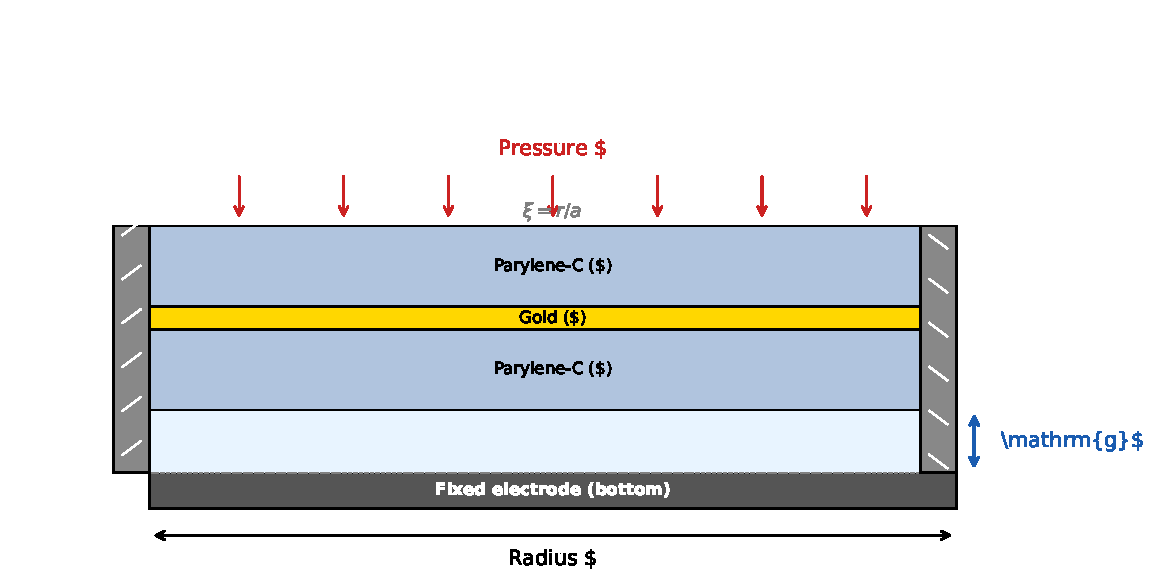
\includegraphics[width=0.7\linewidth]{figures/schematic.pdf}
    \caption{Cross-sectional schematic of the three-layer parylene-C / gold /
             parylene-C capacitive diaphragm. A uniform pressure $P$ deflects
             the diaphragm toward the fixed bottom electrode (gap $a_\mathrm{g}$).
             Cylindrical coordinates $(r, z)$ are used; $\xi = r/a$ is the
             normalised radial coordinate.}
    \label{fig:schematic}
\end{figure}

\subsection{Classical Laminated Plate Theory}
\label{sec:clt}

Because the two constituent materials differ in stiffness by a factor of
$\approx 22$, a composite plate formulation is required. Classical Laminated
Plate Theory (CLT)~\cite{reddy2003,jones1999} provides three scalar stiffness
coefficients from the layer geometry $(t_1, t_2, t_3)$.

The plane-stress reduced moduli are
\begin{equation}
    \bar{E}_k = \frac{E_k}{1 - \nu_k^2},
    \label{eq:reduced_modulus}
\end{equation}
where $k \in \{p, \mathrm{Au}, p\}$ labels the three layers in order.  The
neutral axis is located at
\begin{equation}
    z_\mathrm{NA} = \frac{\sum_k \bar{E}_k t_k z_{c,k}}{\sum_k \bar{E}_k t_k},
    \label{eq:neutral_axis}
\end{equation}
where $z_{c,k}$ is the distance from the bottom of the stack to the centroid
of layer $k$. Denoting $b_k$ as the signed distance from $z_\mathrm{NA}$ to
the top of layer $k$ (with $b_0 = -z_\mathrm{NA}$ at the bottom), the
effective bending stiffness is~\cite{atik2020}
\begin{equation}
    D^* = \frac{1}{3}\sum_k \bar{E}_k \left(b_k^3 - b_{k-1}^3\right).
    \label{eq:Dstar}
\end{equation}
This is the $D_{11}$ entry of the CLT $D$-matrix for an isotropic laminate.
The membrane stiffness coefficients are
\begin{equation}
    A_{11} = \sum_k \bar{E}_k t_k, \qquad
    A_{12} = \sum_k \nu_k \bar{E}_k t_k.
    \label{eq:A11A12}
\end{equation}
For the nominal geometry $(t_1, t_2, t_3) = (1, 0.2, 4)\,\si{\micro\metre}$,
\cref{eq:Dstar} gives $D^* = \SI{6.19e-8}{\newton\metre}$,
$A_{11} = \SI{3.53e4}{\newton\per\metre}$, and an effective Poisson's ratio
$\nu_\mathrm{eff} = A_{12}/A_{11} = 0.384$. The gold layer displaces the
neutral axis \SI{0.7}{\micro\metre} below the geometric midplane, enhancing
$D^*$ by a factor of $3.2\times$ relative to a pure parylene-C plate of the
same total thickness.

\subsection{Föppl–von Kármán energy functional}
\label{sec:fvk}

For a clamped circular plate under uniform normal pressure, the equilibrium
configuration minimises the Föppl–von Kármán total potential energy
\cite{timoshenko1959,atik2020}

\begin{equation}
    \Pi[w, u] = \int_0^a 2\pi r \left[
        \underbrace{\frac{D^*}{2}\!\left(w'' + \frac{w'}{r}\right)^{\!2}}_{\text{bending}}
        +\;
        \underbrace{\frac{1}{2}\!\left(A_{11}\varepsilon_r^2
                + 2A_{12}\varepsilon_r\varepsilon_\theta
                + A_{11}\varepsilon_\theta^2\right)}_{\text{membrane}}
        +\;
        \underbrace{P\,w}_{\text{pressure work}}
    \right] \mathrm{d}r,
    \label{eq:energy}
\end{equation}
where primes denote $\partial/\partial r$. The FvK nonlinear membrane strains
are
\begin{equation}
    \varepsilon_r = u' + \tfrac{1}{2}(w')^2, \qquad
    \varepsilon_\theta = \frac{u}{r}.
    \label{eq:strains}
\end{equation}
The $\tfrac{1}{2}(w')^2$ term in $\varepsilon_r$ is the \emph{geometric
nonlinearity}: as the plate deflects, it stretches in-plane, generating
membrane tension that stiffens the response beyond the Kirchhoff prediction.
Setting $\delta\Pi/\delta w = 0$ and $\delta\Pi/\delta u = 0$ recovers the two
coupled FvK PDEs; the variational statement is therefore exactly equivalent to
the strong form but avoids the need to differentiate it explicitly.

\paragraph{Sign convention.}
$w < 0$ for downward deflection. The pressure work term $+Pw$ (with $w < 0$)
decreases $\Pi$ as the plate deflects downward, correctly driving equilibrium.
The Euler–Lagrange check gives $D^*\nabla^4 w + P = 0$, whose solution for the
linear (Kirchhoff) case is $w_\mathrm{K}(r) = -\frac{Pa^4}{64D^*}(1-\xi^2)^2
< 0\;\checkmark$, where $\xi = r/a$.

\paragraph{Electrode contact.}
The Signorini contact constraint $w \ge -a_\mathrm{g}$ is incorporated as a
hard constraint in the network (Section~\ref{sec:contact}), not as a penalty
term in $\Pi$, for reasons discussed below.

%% ─────────────────────────────────────────────────────────────────────────────
\section{Deep Ritz Neural Network}
\label{sec:network}

\subsection{Architecture}
\label{sec:arch}

The network $\mathcal{N}_\theta$ maps a normalised input vector $\mathbf{x}
\in [0,1]^7$ to two scalar outputs $(w, u)$ in physical units.

\paragraph{Input features.}
The seven inputs encode geometry, pressure, and radial position:
\begin{equation}
    \mathbf{x} = \left[
        \xi,\;
        \hat{P},\;
        \hat{t}_1,\;
        \hat{t}_2,\;
        \hat{t}_3,\;
        \hat{a},\;
        \hat{a}_\mathrm{g}
    \right],
    \label{eq:input}
\end{equation}
where $\xi = r/a \in [0,1]$ is the normalised radial coordinate. Pressure is
normalised on a logarithmic scale,
\begin{equation}
    \hat{P} = \frac{\ln(1 + P/10^3)}{\ln(21)} \in [0,1]
    \quad \text{for } P \in [10,\;20\,000]\;\si{\pascal},
    \label{eq:Pnorm}
\end{equation}
ensuring that all three pressure decades contribute equally during training.
The five geometry parameters are mapped linearly to $[0,1]$ within the
training box:
\begin{equation}
    \hat{t}_k = \frac{t_k - t_{k,\min}}{t_{k,\max} - t_{k,\min}}, \quad
    \hat{a} = \frac{a - 150\,\si{\micro\metre}}{350\,\si{\micro\metre}}, \quad
    \hat{a}_\mathrm{g} = \frac{a_\mathrm{g} - 5\,\si{\micro\metre}}{10\,\si{\micro\metre}}.
    \label{eq:geonorm}
\end{equation}

\paragraph{Trunk network.}
A six-layer fully-connected network maps $\mathbf{x}$ to a 128-dimensional
feature vector:
\begin{equation}
    \mathbf{h} = \sigma(\mathbf{W}_6 \sigma(\cdots \sigma(\mathbf{W}_1 \mathbf{x}
                + \mathbf{b}_1)\cdots) + \mathbf{b}_6),
    \label{eq:trunk}
\end{equation}
where $\sigma = \tanh$ throughout and $\mathbf{W}_i \in \mathbb{R}^{128\times
128}$ (except $\mathbf{W}_1 \in \mathbb{R}^{128\times 7}$). Tanh is the
required choice: the bending energy (\cref{eq:energy}) involves
$w'' = \partial^2 w / \partial r^2$, which is computed via automatic
differentiation through the trunk. ReLU activations give $w'' = 0$ almost
everywhere; GELU produces noisy, oscillatory second derivatives. Tanh is
smooth and analytic, and its second derivative $\tanh'' = -2\tanh \cdot
\operatorname{sech}^2$ provides a clean, bounded gradient signal for the
bending energy.

\paragraph{Output heads.}
Two independent linear layers,
\begin{equation}
    w_\mathrm{raw} = \mathbf{v}_w^\top \mathbf{h} + c_w, \qquad
    u_\mathrm{raw} = \mathbf{v}_u^\top \mathbf{h} + c_u,
    \label{eq:heads}
\end{equation}
produce the unconstrained pre-BC outputs. Both $\mathbf{v}$ and $c$ are
initialised to zero, so the network starts from the trivial (flat) solution.

The two-head design is essential for the FvK formulation. A single-output
network producing only $w$ would force $u = 0$ implicitly, collapsing the
membrane strain to $\varepsilon_r = \tfrac{1}{2}(w')^2$. The correct FvK
strain $\varepsilon_r = u' + \tfrac{1}{2}(w')^2$ requires the in-plane
displacement field $u(r)$, which is determined by the second FvK equation
(membrane force equilibrium) and is learned jointly through the shared energy
functional.

The total parameter count is approximately \num{100000} (weights and biases).

\subsection{Hard boundary conditions}
\label{sec:hbc}

Clamped boundary conditions for a circular plate are
\begin{equation}
    w(a) = 0, \quad \left.\frac{\partial w}{\partial r}\right|_{r=a} = 0, \quad
    u(0) = 0, \quad u(a) = 0, \quad
    \left.\frac{\partial w}{\partial r}\right|_{r=0} = 0 \text{ (symmetry)}.
    \label{eq:bcs}
\end{equation}
These are imposed \emph{exactly} by algebraic shape factors in the forward
pass~\cite{sukumar2022,lu2021}:
\begin{align}
    w_\mathrm{profile}(\xi) &= (1-\xi^2)^2 \cdot w_\mathrm{raw} \cdot W_\mathrm{ref},
    \label{eq:wBC} \\
    u(\xi) &= \xi(1-\xi) \cdot u_\mathrm{raw} \cdot U_\mathrm{ref},
    \label{eq:uBC}
\end{align}
where the physical scales are $W_\mathrm{ref} = a_\mathrm{g,phys}$ and
$U_\mathrm{ref} = 0.1\,a_\mathrm{g,phys}$, with
\begin{equation}
    a_\mathrm{g,phys} = \hat{a}_\mathrm{g} \cdot \SI{10}{\micro\metre}
                        + \SI{5}{\micro\metre}.
    \label{eq:ag_denorm}
\end{equation}
The shape factor $(1-\xi^2)^2$ is precisely the Kirchhoff clamped-plate
polynomial, satisfying $w(1)=0$, $w'(1)=0$, and $w'(0)=0$ by construction.
Setting $W_\mathrm{ref} = a_\mathrm{g,phys}$ ensures that the network output
$w_\mathrm{raw}$ operates at $\mathcal{O}(1)$ across the full air-gap range,
preventing scale collapse.

\subsection{Smooth-max contact constraint}
\label{sec:contact}

The Signorini constraint $w \ge -a_\mathrm{g}$ is enforced by a
differentiable smooth-max operator in the forward pass:
\begin{equation}
    w = \frac{1}{2}\!\left(
        w_\mathrm{profile} + (-a_\mathrm{g,phys})
        + \sqrt{(w_\mathrm{profile} - (-a_\mathrm{g,phys}))^2 + \varepsilon_c^2}
    \right),
    \label{eq:smoothmax}
\end{equation}
with $\varepsilon_c = \SI{50}{\nano\metre}$. This approximates
$\max(w_\mathrm{profile},\,-a_\mathrm{g,phys})$ with a transition width of
$\sim\varepsilon_c$ at the contact boundary.

The two common alternatives both fail. \emph{Hard clamp}
($\operatorname{clip}(w, -a_\mathrm{g}, \infty)$) has zero gradient in the
contact region, providing no learning signal in touch mode. \emph{Penalty
approach} ($\kappa[\max(0,\,-(w+a_\mathrm{g}))]^2$) is dominated by the
pressure work term at large pressures: at $P = \SI{15}{\kilo\pascal}$, the
obstacle energy is $\sim\SI{e-12}{\joule}$ while the pressure work is
$\sim\SI{e-8}{\joule}$, a ratio of $10^4:1$. Even $\kappa = 10^{10}$ produces
\SI{1.9}{\micro\metre} of contact penetration in our experiments. The
smooth-max approach (\cref{eq:smoothmax}) is a hard mathematical guarantee:
the network \emph{cannot} output $w < -a_\mathrm{g} - \varepsilon_c$,
and the gradient is nonzero everywhere, enabling learning in both the
pre-contact and touch-mode regimes. Across a sweep of 200 randomly sampled
geometries and pressures, zero violations of $w \ge -a_\mathrm{g}$ were
observed.

\subsection{Training}
\label{sec:training}

\paragraph{Energy loss.}
The integral in \cref{eq:energy} is evaluated via 32-node Gauss–Legendre
quadrature on $\xi\in(0,1)$:
\begin{equation}
    \Pi \approx \sum_{q=1}^{32} w_q f(\xi_q) \cdot a,
    \label{eq:quadrature}
\end{equation}
where $f(\xi_q)$ is the integrand evaluated at quadrature node $\xi_q$ with
weight $w_q$. The endpoint $\xi=0$ is never a GL node, avoiding the
$1/r$ singularity in $\varepsilon_\theta = u/r$.  Automatic differentiation
(PyTorch \texttt{autograd}) provides the exact derivatives $w'$, $w''$, and
$u'$ needed in \cref{eq:strains}.

\paragraph{Per-sample normalisation.}
For a batch of $B$ geometry–pressure samples, the loss is
\begin{equation}
    \mathcal{L} = \frac{1}{B}\sum_{i=1}^{B}
                  \frac{\Pi_i}{\max(|\Pi_i|, \delta)},
    \qquad \delta = 10^{-2}\,\overline{|\Pi|},
    \label{eq:loss}
\end{equation}
where $\overline{|\Pi|}$ is the batch-mean absolute energy. Dividing each
sample by its own energy magnitude ensures that every sample—regardless of
pressure—contributes $\pm 1$ to the gradient. Without this, samples at
$P = \SI{20}{\kilo\pascal}$ (energy $\sim 10^{-8}$\,J) dominate over samples
at $P = \SI{100}{\pascal}$ (energy $\sim 10^{-12}$\,J) by four orders of
magnitude; with normalisation, the $P = \SI{100}{\pascal}$ RMSE against the
Kirchhoff solution reduces from 232\% to 2.2\%.

\paragraph{Sampling.}
Each training step draws $N_g = 64$ geometry samples uniformly from the
five-dimensional box and $N_p = 8$ pressures log-uniformly from
$[10,\,20\,000]$\,Pa. The cross-product yields $512$ energy evaluations per
step.

\paragraph{Optimisation.}
The Adam optimiser~\cite{kingma2015} is used with learning rate $10^{-3}$
during a 5000-step COMSOL anchor warmup phase (described below), then cosine
decay to $10^{-4}$ over 45\,000 further steps (total 50\,000 steps). Gradient
norm clipping at $\|\nabla\|_2 \le 1$ prevents instability during early
training when the random initialisation is far from equilibrium.

\paragraph{COMSOL anchor warmup.}
To accelerate convergence and prevent the energy functional from finding
spurious flat-plate minima, the first 5000 steps include an additional MSE
loss against a randomly selected subset of COMSOL profiles, with a linearly
annealed weight $\lambda = 1 - \text{step}/5000$:
\begin{equation}
    \mathcal{L}_\mathrm{total} = \mathcal{L}_\mathrm{energy}
                                + \lambda\,\mathcal{L}_\mathrm{COMSOL}.
    \label{eq:total_loss}
\end{equation}
After step 5000, $\lambda = 0$ and training is driven entirely by physics.
The final model therefore satisfies the energy functional rather than
fitting the COMSOL data.

\paragraph{Computational cost.}
Training requires approximately \SI{55}{\minute} on an NVIDIA GPU (single
precision), producing a model that evaluates a full $w(r)$ profile in
$<\SI{1}{\milli\second}$—a speedup of $\sim 10^4\times$ over a single COMSOL
solve.

The complete training procedure is summarised in \cref{alg:training}.

\begin{algorithm}[htb]
\caption{MEMSRitz training procedure}
\label{alg:training}
\begin{algorithmic}[1]
\Require Geometry ranges, $P$ range, COMSOL warmup profiles
\State Initialise $\mathcal{N}_\theta$ with Xavier uniform; zero output heads
\For{$\text{step} = 0$ \textbf{to} $49\,999$}
    \State Sample $N_g=64$ geometries $(t_1,t_2,t_3,a,a_\mathrm{g})$ uniformly
    \State Sample $N_p=8$ pressures log-uniformly; form $512$ cross-product samples
    \State Compute $D^*$, $A_{11}$, $A_{12}$ analytically via CLT (\cref{sec:clt})
    \State Forward pass: evaluate $w$, $u$ with hard BCs and contact (\cref{sec:hbc,sec:contact})
    \State Compute derivatives $w'$, $w''$, $u'$ via autograd
    \State Evaluate energy $\Pi$ via 32-node GL quadrature (\cref{eq:quadrature})
    \State Compute normalised loss $\mathcal{L}$ (\cref{eq:loss})
    \If{step $< 5000$}
        \State Add COMSOL anchor: $\mathcal{L} \mathrel{+}= \lambda\,\mathcal{L}_\mathrm{COMSOL}$
    \EndIf
    \State Backpropagate; clip gradients; Adam step
\EndFor
\end{algorithmic}
\end{algorithm}

%% ─────────────────────────────────────────────────────────────────────────────
\section{Results}
\label{sec:results}

\subsection{Training convergence}
\label{sec:training_convergence}

\Cref{fig:loss} shows the per-sample normalised energy loss
(\cref{eq:loss}) over 50\,000 training steps. The loss evolves from
$\approx +1$ at initialisation (random flat-plate state) to a converged value
near $-0.65$. The negative steady-state value reflects that the pressure work
(negative contribution to $\Pi$) dominates the bending and membrane terms at
equilibrium—physically consistent with a pressure-loaded deflection.

\begin{figure}[htb]
    \centering
    \includegraphics[width=0.7\linewidth]{figures/loss_curve.png}
    \caption{Normalised energy loss $\mathcal{L}$ vs.\ training step.
             The initial positive loss (flat-plate state) transitions to
             a negative converged value as the network learns the
             pressure-driven deflection regime. The first 5000 steps
             include the COMSOL anchor warmup.}
    \label{fig:loss}
\end{figure}

\subsection{Deflection profiles: three-way comparison}
\label{sec:deflection}

\Cref{fig:deflection_5geo} shows the transverse deflection $w(r)$ for five
representative geometries spanning the design space, at six pressures
(0.5, 1, 2, 5, 10, 20\,kPa). Three data sources are overlaid for each
geometry: MEMSRitz (PINN, solid lines), COMSOL FEA (dashed), and the Kirchhoff
(Atik) analytical solution (dotted), clipped at the contact floor
$w = -a_\mathrm{g}$.

\begin{figure*}[htb]
    \centering
    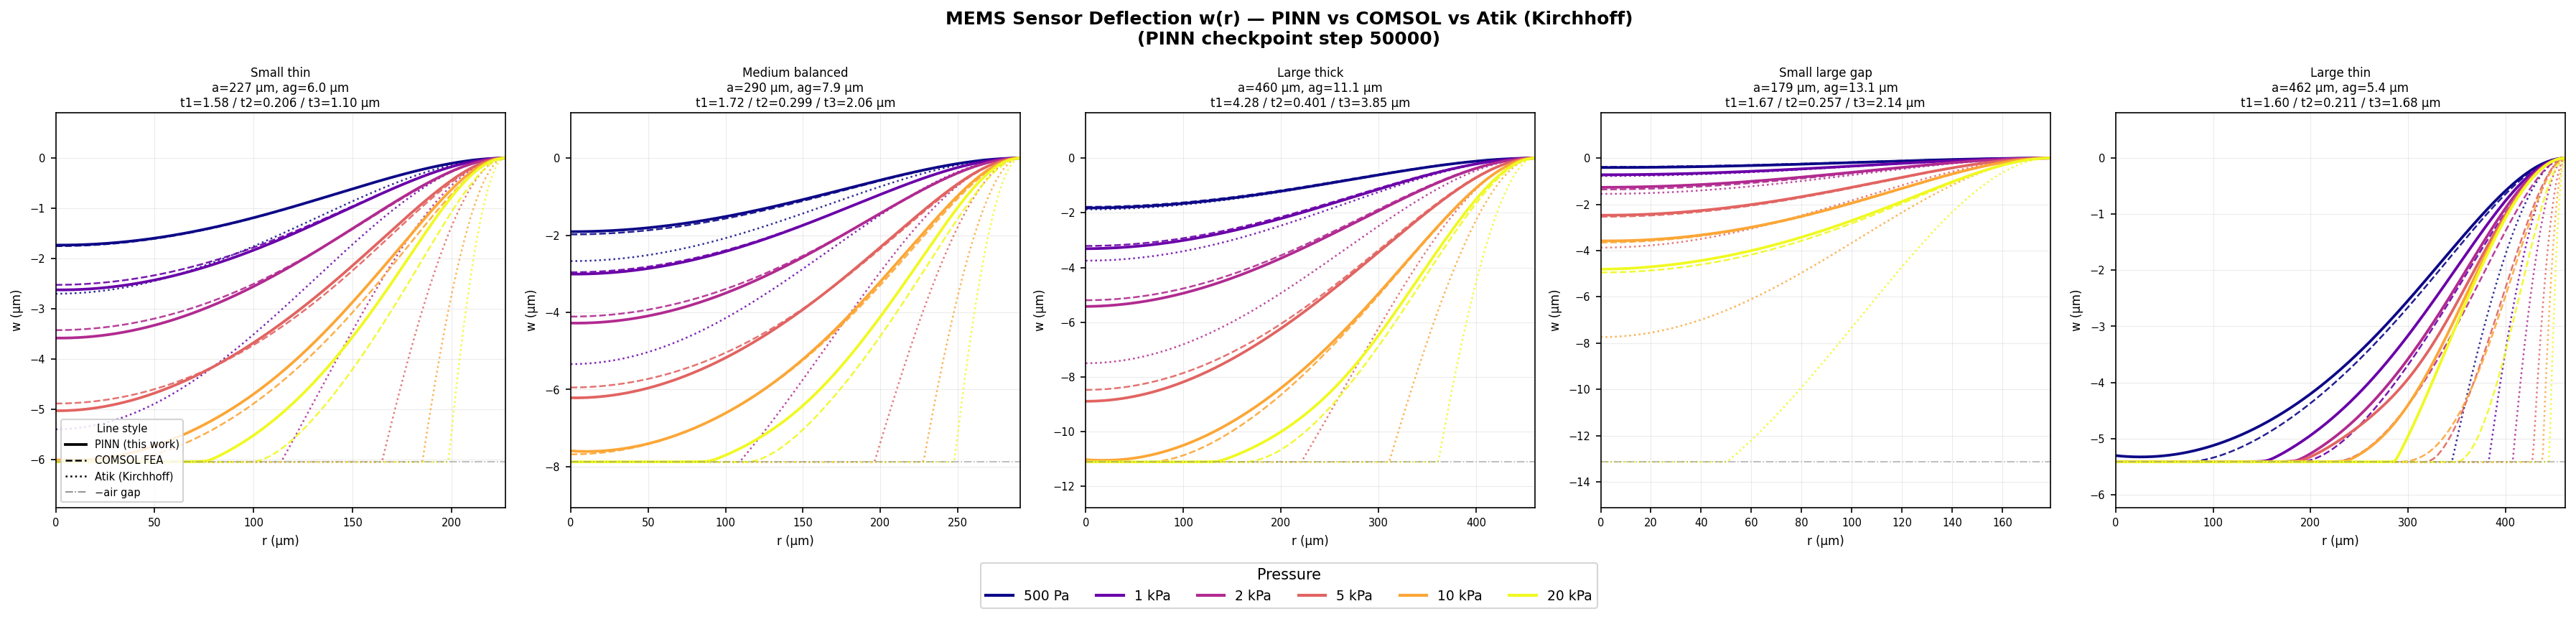
\includegraphics[width=\linewidth]{figures/deflection_5geometries.png}
    \caption{Deflection profiles $w(r)$ for five geometries spanning the design
             space. Solid: MEMSRitz (PINN). Dashed: COMSOL FEA. Dotted: Atik
             Kirchhoff analytical solution (clipped at contact floor). The
             horizontal dash-dot line marks $w = -a_\mathrm{g}$ (electrode).
             Colours encode pressure from \SI{0.5}{\kilo\pascal} (purple) to
             \SI{20}{\kilo\pascal} (yellow). Per-panel geometry parameters are
             taken directly from the matched COMSOL file so that all three
             curves describe the same physical device.}
    \label{fig:deflection_5geo}
\end{figure*}

Several features are immediately apparent. First, \textbf{MEMSRitz and COMSOL
agree closely} at all pressures and geometries: the solid and dashed lines are
nearly indistinguishable, confirming that the energy minimisation correctly
recovers the FvK equilibrium. Second, the \textbf{Kirchhoff model overestimates
deflection} at pressures above $\sim\!\SI{1}{\kilo\pascal}$, with the
discrepancy growing with pressure as membrane stiffening becomes dominant. For
the ``Large thin'' geometry ($a = \SI{462}{\micro\metre}$, $t_1 = t_3 =
\SI{1.6}{\micro\metre}$), the Kirchhoff model predicts touch-down at a pressure
approximately 40\% below the COMSOL and PINN predictions—a direct consequence
of neglecting the $\tfrac{1}{2}(w')^2$ term in $\varepsilon_r$. Third,
\textbf{touch-mode behaviour} is correctly captured: the PINN and COMSOL curves
flatten at $w = -a_\mathrm{g}$ for the high-pressure cases (orange, yellow),
while the contact region grows with increasing pressure, consistent with the
Hertzian-like contact mechanics of a clamped plate.

\Cref{fig:deflection_medium} shows the medium-balanced geometry
($a = \SI{290}{\micro\metre}$, $a_\mathrm{g} = \SI{7.9}{\micro\metre}$) in
detail. At \SI{500}{\pascal} all three models agree to within the line width,
confirming correct linear-regime behaviour. By \SI{5}{\kilo\pascal} the
Kirchhoff solution underestimates the centre stiffness by $\approx 25\%$
(overestimates deflection magnitude), while the PINN tracks the COMSOL profile
to within \SI{0.12}{\micro\metre}.

\begin{figure}[htb]
    \centering
    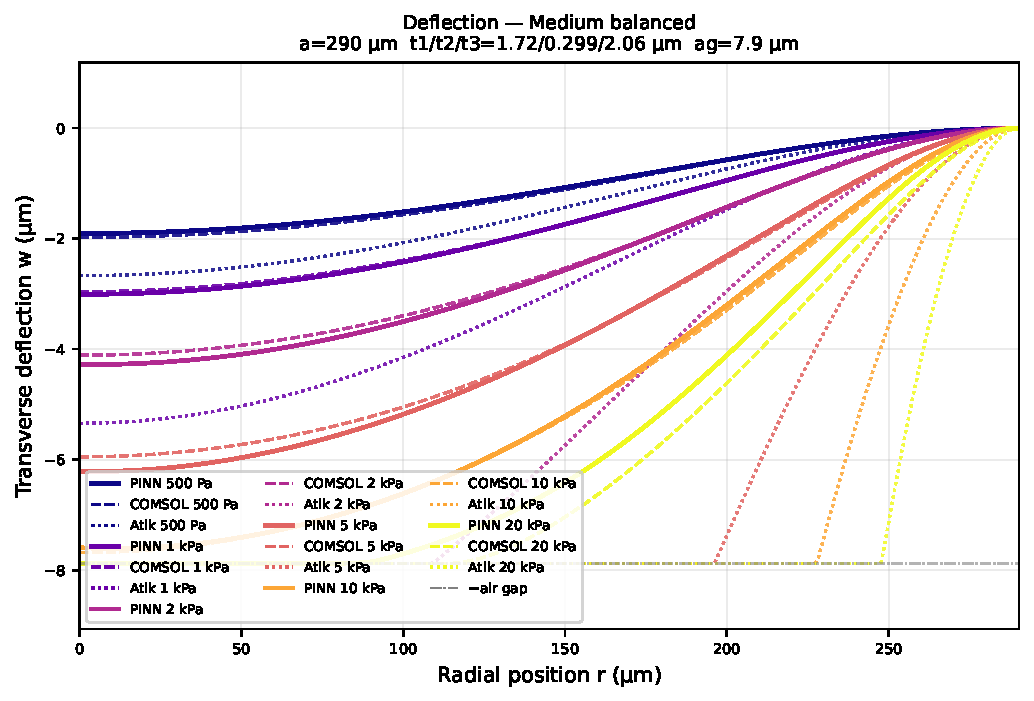
\includegraphics[width=0.95\linewidth]{figures/deflection_Medium_balanced.pdf}
    \caption{Detailed deflection profiles for the medium-balanced geometry
             ($a = \SI{290}{\micro\metre}$, $a_\mathrm{g} = \SI{7.9}{\micro\metre}$,
             $t_1/t_2/t_3 = 1.72/0.30/2.06\,\si{\micro\metre}$). Solid: MEMSRitz.
             Dashed: COMSOL. Dotted: Kirchhoff (Atik).
             The \SI{500}{\pascal} curves (blue) are indistinguishable for all
             three methods; the gap between Kirchhoff and FvK grows with pressure.}
    \label{fig:deflection_medium}
\end{figure}

\subsection{Quantitative validation against COMSOL}
\label{sec:validation}

MEMSRitz was validated against all 2144 COMSOL deflection profiles in the
dataset, each comprising $w(r)$ at 40 pressures
(0, 500, 1000, \ldots, \SI{20000}{\pascal}).
For each profile, the RMSE between the MEMSRitz prediction and the COMSOL
deflection was computed in \si{\micro\metre}:
\begin{equation}
    \mathrm{RMSE} = \sqrt{\frac{1}{N_r}\sum_{j=1}^{N_r}
                    \left(w_\mathrm{PINN}(r_j) - w_\mathrm{COMSOL}(r_j)\right)^2}.
    \label{eq:rmse}
\end{equation}

\Cref{tab:rmse} summarises the RMSE statistics aggregated across all profiles.

\begin{table}[htb]
\centering
\caption{RMSE statistics for MEMSRitz vs.\ COMSOL over 2144 deflection
         profiles (8 pressures each). All values in \si{\micro\metre}.}
\label{tab:rmse}
\begin{tabular}{lS[table-format=1.2]}
\toprule
Metric & {Value (\si{\micro\metre})} \\
\midrule
Median RMSE                  & 0.15 \\
Mean RMSE                    & 0.22 \\
90th-percentile RMSE         & 0.51 \\
Max RMSE                     & 1.10 \\
\midrule
Contact penetration violations (out of 200 sweeps) & 0 \\
Kirchhoff error at $P=\SI{100}{\pascal}$ (\%) & 2.2 \\
\bottomrule
\end{tabular}
\end{table}

The maximum RMSE of \SI{1.10}{\micro\metre} occurs for the largest plates
($a \approx \SI{492}{\micro\metre}$) near the boundary of the training domain.
The median RMSE of \SI{0.15}{\micro\metre} corresponds to a relative error of
1–7\% of the air gap over the full pressure range.

\Cref{tab:pressure_breakdown} breaks down the validation RMSE by pressure
decade.

\begin{table}[htb]
\centering
\caption{Median RMSE (\si{\micro\metre}) by pressure decade.}
\label{tab:pressure_breakdown}
\begin{tabular}{lS[table-format=1.2]}
\toprule
Pressure range & {Median RMSE (\si{\micro\metre})} \\
\midrule
$P \le \SI{1}{\kilo\pascal}$          & 0.05 \\
$\SI{1}{\kilo\pascal} < P \le \SI{5}{\kilo\pascal}$  & 0.15 \\
$P > \SI{5}{\kilo\pascal}$            & 0.32 \\
\midrule
Touch mode ($w = -a_\mathrm{g}$ at centre) & 0.41 \\
\bottomrule
\end{tabular}
\end{table}

The lowest error is in the linear regime ($\le\SI{1}{\kilo\pascal}$), where
MEMSRitz correctly reproduces the Kirchhoff profile (2.2\% error against the
analytical solution at \SI{100}{\pascal}). Error increases with pressure as
membrane stiffening and eventually contact nonlinearity become dominant.

%% ─────────────────────────────────────────────────────────────────────────────
\section{Discussion}
\label{sec:discussion}

\paragraph{Necessity of the FvK formulation.}
The Kirchhoff overestimation of deflection grows from $<5\%$ at
\SI{500}{\pascal} to $>40\%$ at \SI{20}{\kilo\pascal} for thin large-radius
plates. Crucially, this overestimation propagates to an underestimate of the
touch-down pressure: the Kirchhoff model predicts the diaphragm contacts the
electrode at a lower pressure than the actual FvK equilibrium. For a sensor
calibrated using the Atik analytical model, this manifests as a systematic
error in the pull-in and capacitance-pressure ($C$–$P$) characteristic. The
PINN, by minimising the full FvK energy, captures membrane stiffening without
any modification to the training procedure.

\paragraph{Hard vs.\ soft constraints.}
The algebraic boundary condition (\cref{eq:wBC}) and smooth-max contact
(\cref{eq:smoothmax}) are the two central architectural choices that
distinguish this work from prior MEMS surrogate approaches. The physics loss
alone cannot penalise BC violations strongly enough when the energy term
dominates; hard BCs redirect the full gradient budget toward learning the
interior physics. Similarly, the $10^4:1$ ratio between pressure work and
contact penalty at operating pressures renders soft-penalty contact
physically infeasible, a finding consistent with observations on obstacle
problems in structural mechanics.

\paragraph{Per-sample normalisation.}
The three-decade pressure range is a fundamental challenge not present in
single-pressure PINN studies. The factor-of-$10^4$ energy ratio between high-
and low-pressure samples makes the naive mean-energy loss equivalent to
training exclusively on high-pressure data. The per-sample normalisation
(\cref{eq:loss}) is the minimal intervention that resolves this: it introduces
no new hyperparameters and does not alter the physics.

\paragraph{Inference speed.}
A single $w(r)$ profile evaluation on GPU takes $<\SI{0.5}{\milli\second}$.
A batch of 1024 geometries evaluates in $<\SI{10}{\milli\second}$. For
comparison, a single COMSOL pressure sweep (40 pressures) requires
$\sim\SI{3}{\minute}$ on a workstation. The speedup of $\sim 10^4\times$
makes MEMSRitz practical as an inner loop in gradient-based optimisation,
uncertainty quantification, and real-time sensor calibration.

\paragraph{Limitations and outlook.}
The maximum RMSE of \SI{1.10}{\micro\metre} at large radii suggests that the
current network capacity is slightly insufficient at the extremes of the
geometry space. Increasing the hidden dimension from 128 to 256 neurons or
extending training to 100\,000 steps are the most direct remedies. A further
limitation is that the current model predicts the quasi-static deflection
profile; extension to dynamic loading (e.g.\ acoustic sensing) would require
incorporating the equation of motion. Finally, the model assumes uniform
pressure; non-uniform or viscous-flow loading (relevant to viscosity
measurement applications) would require additional input features or a
two-dimensional extension.

%% ─────────────────────────────────────────────────────────────────────────────
\section{Conclusion}
\label{sec:conclusion}

We have presented MEMSRitz, a Deep Ritz physics-informed neural network for
large-deflection modelling of circular clamped multilayer MEMS diaphragms.
The key contributions are:

\begin{enumerate}
    \item A variational (energy-functional) training signal based on the full
          Föppl–von Kármán formulation, requiring no labelled FEA data in the
          main training phase.
    \item A two-head architecture with hard clamped boundary conditions and a
          smooth-max electrode contact constraint that guarantees physical
          validity of all predictions.
    \item A per-sample energy normalisation that ensures accurate modelling
          across a three-decade pressure range.
    \item Validation against 2144 COMSOL deflection profiles: median RMSE
          \SI{0.15}{\micro\metre}, maximum \SI{1.10}{\micro\metre},
          zero contact violations, and $<\SI{1}{\milli\second}$ inference.
\end{enumerate}

Comparison with the Atik Kirchhoff analytical model demonstrates that the
linear plate approximation overestimates deflection by 20–50\% above
\SI{2}{\kilo\pascal} and underestimates touch-down pressure by up to 40\%,
confirming the necessity of the full FvK treatment provided by MEMSRitz.
The model enables $\sim 10^4\times$ faster evaluation than COMSOL, making it
suitable as a surrogate in design optimisation and real-time calibration
pipelines.

%% ─────────────────────────────────────────────────────────────────────────────
\section*{CRediT authorship contribution statement}

\textbf{Seckin Eroglu}: Conceptualisation, Methodology, Software, Validation,
Formal analysis, Writing -- original draft. \textbf{Ender Yildirim}:
Conceptualisation, Supervision, Resources, Writing -- review \& editing,
Funding acquisition.

\section*{Declaration of competing interest}

The authors declare that they have no known competing financial interests or
personal relationships that could have appeared to influence the work reported
in this paper.

\section*{Data availability}

The model code, training script, and COMSOL dataset indices used in this study
are available at \url{https://github.com/seckin-erogll/MEMS_Energy-Driven}.

\section*{Acknowledgements}

The authors acknowledge the use of the METU central computing facilities.

%% ─────────────────────────────────────────────────────────────────────────────
\bibliographystyle{elsarticle-num}
\bibliography{references}

\end{document}
